%!TEX root = ../lectures_olympics.tex

\chapter{交流电路}
\begin{wrapfigure}{o}{6cm}
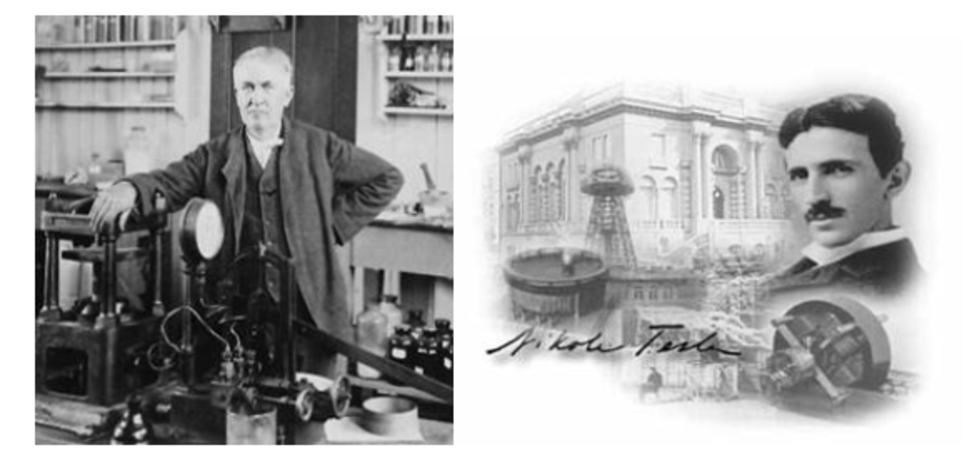
\includegraphics[width=6cm]{images/mag-20.pdf} 
\caption{爱迪生(\textit{T. Edison})和特斯拉(\textit{N. Tesla})之间上演了一出著名的直流交流电之争}
\end{wrapfigure}
利用外力推动一个线圈在磁场当中转动,根据电磁感应现象可使线圈当中产生周期性变化的感生电动势,在电路当中就有了大小和方向交替变化的电流,称之为{\heiti 交流电}(alternating current, AC)。
交流电路与普通化学电池做为电源的直流电路有很大的不同,在发现交流电的早期人们曾经经历了交流电和直流电之争,最终的结果大家都知道,交流电以其巨大的优势战胜了直流电,成为近代人类生活的主要电源。
\section{交流电、交流发电机}
在电磁感应一章当中我们已知,当一个面积为$S$的线圈在磁感应强度为$B$的匀强磁场当中以角速度$\omega$做匀速转动时,由于切割磁感线,或者说线圈内的磁通量随时间发生变化,线圈中会有随时间而变的感应电动势:
\begin{equation}
\mathcal{E}(t) =U(t)= \omega BS\cos\omega t  = U_0\cos\omega t.
\end{equation}
其中$U_0$称为交流电的电压极大值,与简谐振动相类比,$\omega$称为交流电的角频率。
这样交流电的周期和频率将分别为
\begin{equation}
T = \frac{2\pi}{\omega},\qquad f = \frac{1}{T} = \frac{\omega}{2\pi}.
\end{equation}
这就是最简单的{\heiti 交流发电机}(AC generator)的模型,当发电机与一个定值电阻相连接时回路中的电流由欧姆定律
\begin{equation}
I(t) = \frac{U(t)}{R} = \frac{U_0}{R}\cos\omega t.
\end{equation}
交流电路中$U(t)$、$I(t)$分别称做电压和电流的{\heiti 瞬时值}(instantaneous value),从上面的关系式可以看出,瞬时值看上去和极大值为振幅、给定频率的简谐振动非常类似。

众所周知,我国民用的交流电的频率为$50\unit{Hz}$,也就是说电压将在一秒之内达到50次极大值,所以用瞬时值来描写电路的特性显得很麻烦也没有实际意义。
为此引入交流电路的各种平均值是有必要的,因为在实际使用中最关心的是电器的功率,为此目的定义交流电的{\heiti 有效电压}(effetive voltage),当在交流电路中接入一个定值电阻$R$时,该电阻的热功率的瞬时值
\begin{equation}
P(t) = \frac{U(t)^2}{R} = \frac{U_0^2}{R}\cos^2\omega t,
\end{equation}
由于交流电的频率非常高,所以实际上消耗在该电阻上的热功率是瞬时热功率的时间平均值:
\begin{equation}
\overline{P} = \frac{1}{T}\int_0^TP(t) = \frac{1}{2}\frac{U_0^2}{R}  = \frac{(\frac{1}{\sqrt{2}}U_0)^2}{R}= \frac{U_{eff}^2}{R}
\end{equation}
从中可以看出,交流电中电阻上的热功率等同于将它连入$U_{eff} = U_0/\sqrt{2}$的直流电路中相当,将$U_{eff}$称为交流电的有效电压,有时根据其计算方式也称为{\heiti 均方根电压}(root mean square voltage, $U_{rms}$)。
我们知道,我国的民用电路的有效电压为$220\unit{V}$,而在美国、日本等国家则是$110\unit{V}$,这一点在旅行中要特别注意。
同理可以定义有效电流,和有效电压的计算做类比马上可知有效电流也是电流极大值的$1/\sqrt{2}$,
\begin{equation}
I_{eff} = \frac{1}{\sqrt{2}}I_0.
\end{equation}



%%%%%%%%%%%%%%%%%
\begin{example}
求以下一些非正弦交流电的有效值:

$(1). \text{方波}\qquad \qquad (2). \text{三角波}\qquad \qquad (3). \text{全波整流后的正弦波}\qquad \qquad $
\begin{center}
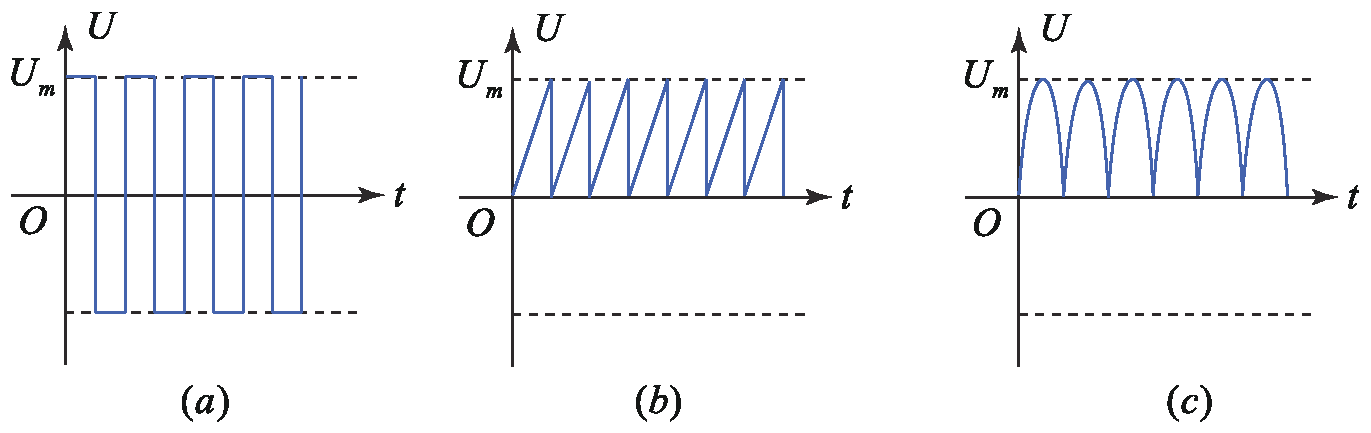
\includegraphics[width = 0.7\textwidth]{images/alt-current-4.pdf} 
\end{center}
\tagged{student}{\vspace*{4cm}}
\begin{taggedblock}{teacher}
\noindent
解析:1.$U=U_m$
\\2.$U=\frac{U_m}{\sqrt{3}}$
\\3.$U=\frac{U_m}{\sqrt{2}}$
\end{taggedblock}
\end{example}
%%%%%%%%%%%%%%%%%%%%%%



%%%%%%%%%%%%%%%%%
\begin{example}

有一交流电压的变化规律为$U = 311\sin (314t)\unit{V}$,若将一辉光电压最小值是$220\unit{V}$的氖管接上此交流电压(只有当瞬时电压大于辉光电压时氖管才会发光),则在1秒内氖管发光的时间是多少。

\tagged{student}{\vspace*{4cm}}
\begin{taggedblock}{teacher}
\noindent
解析:0.5s
\end{taggedblock}
\end{example}
%%%%%%%%%%%%%%%%%%%%%%




%%%%%%%%%%%%%%%%%
\begin{example}
如图所示,常用示波器中的扫描电压$u$随时间$t$变化的图线是
\begin{center}
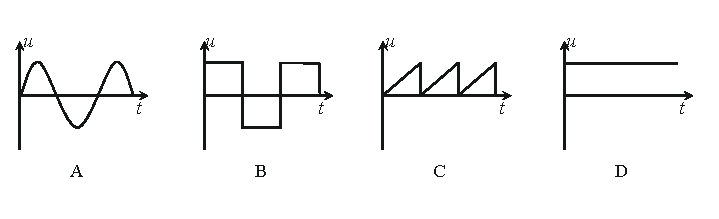
\includegraphics[width = 0.8\textwidth]{images/alt-current-5.pdf} 
\end{center}


\tagged{student}{\vspace*{0cm}}
\begin{taggedblock}{teacher}
\noindent
解析:C
\end{taggedblock}
\end{example}
%%%%%%%%%%%%%%%%%%%%%%


\section{交流电路中的电感和电容}
在直流电路中接入的电感和电容,当电流达到稳定以后它们分别可看成是理想的导线和断路,但在交流电路则不同,由于电流不断地发生变化,它们将产生明显的响应。

\begin{figure}[hb]
\centering
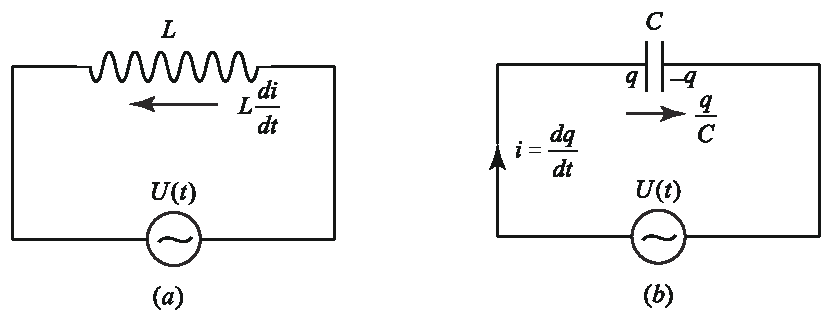
\includegraphics[width=0.7\textwidth]{images/alt-current-1.pdf}
\caption{接入交流电路中的电感和电容,左图箭头表示电动势方向,右图箭头表示电势降方向}
\label{fig:alt-current-1}
\end{figure}


如图\ref{fig:alt-current-1}(a)所示,在路端电压$U = U_0\cos\omega t$的交流电路中接入电感为$L$的线圈,电压的变化会导致回路中电流的变化,而通过电感电流发生变化时由于电磁感应现象电感将产生抵抗电动势,其大小为
\begin{equation}
-L\frac{dI}{dt},
\end{equation}
当最终形成稳定状态以后,线路中电流、电压的变化量应满足:
\begin{equation}
U_0\cos\omega t = L\frac{dI}{dt}
\end{equation}
为使上式成立,可以证明,线路中的电流需要满足
\begin{equation}
I(t) = \frac{U_0}{\omega L}\sin\omega t = \frac{U_0}{\omega L}\cos(\omega t - \frac{\pi}{2}).
\end{equation}
从中可以看出,接入电感以后电流的极大值不但与电感本身的大小$L$有关,还与交流电本身的频率有关,这一点和电阻有很大的不同;第二,接入电感以后电流和电压的相位不再同步,同样的现象在电阻上也是不存在的。
此外,接入电感以后产生的最大电流值可看做是路端电压的极大值除以$\omega L$所得到的结果,它的作用和电阻阻值有着类似的地位,实践上将$\omega L$称为电感的{\heiti 感抗}(inductive reactance),在纯电感交流电路中,电压极大值除以感抗就得到电流的极大值。


同理如图\ref{fig:alt-current-1}(b)中在交流电路中接入一个容值为$C$的电容后,设电容器内充电的瞬时值为$q(t)$,则它产生的电压为$\frac{q(t)}{C}$,它将与路端电压平衡,由于路端电压不断地随时间变换,电容器也处于不断地充电、放电过程中:
\begin{equation}
U(t) = U_0\cos\omega t = \frac{q(t)}{C}.
\end{equation}
当线路处于稳定状态时可以证明,电容带电量必须满足
\begin{equation}
q(t) = U_0 C \cos\omega t,
\end{equation}
而电容的充电和放电是由线路中的电流引起的,这时线路中的电流自然就是电容器所带电量对时间的导数:
\begin{equation}
I(t) = \frac{dq(t)}{dt} = - \omega C U_0\sin\omega t = \frac{U_0}{\frac{1}{\omega C}}\cos(\omega t+\frac{\pi}{2}).
\end{equation}
和电感的情况类似,接入交流电路中的电容器引起的电流极大值也同时与电容值$C$和交流电的频率$\omega$有关,同时也产生$\frac{\pi}{2}$相位差,但是与电感产生的相位差相反。
实践上将电压极大值与电流极大值之间的比值$\frac{1}{\omega C}$称为纯电容电路的{\heiti 容抗}(capacitive reactance),它也有着和电阻类似的作用。


%%%%%%%%%%%%%%%%%
\begin{example}

以下两个交流电路中路端电压均为$U = U_0\cos\omega t$,求线路中电流随时间的变化关系,每个电路中定义取箭头方向为正方向。
\begin{center}
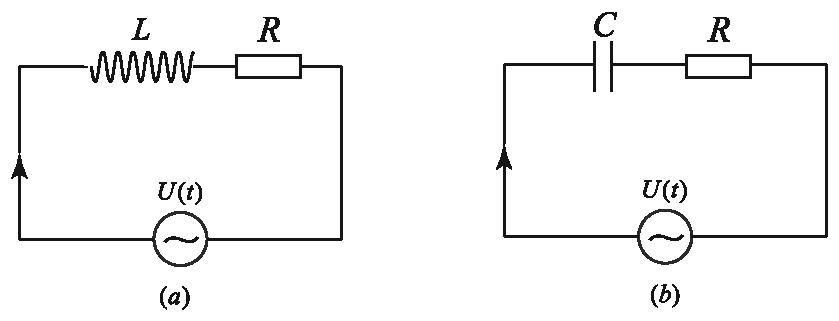
\includegraphics[width = 0.7\textwidth]{images/alt-current-2.pdf}
\end{center}
\tagged{student}{\vspace*{4cm}}
\begin{taggedblock}{teacher}
\noindent
解析:
对于$RL$电路:$I = \frac{U_0}{\sqrt{R^2+\omega^2 L^2}}\cos(\omega t-\varphi)\quad ; \quad \varphi=\arctan \frac{\omega L}{R}$

对于$RC$电路:$I = \frac{U_0}{\sqrt{R^2+\frac{1}{\omega^2 C^2}}}\cos(\omega t+\varphi)\quad ; \quad \varphi=\arctan \frac{1}{\omega CR}$
\end{taggedblock}
\end{example}
%%%%%%%%%%%%%%%%%%%%%%


%%%%%%%%%%%%%%%%%
\begin{example}
如图所示的$LC$回路,初始时刻开关$S$断开,电容器带电$Q_0>0$。
在$t=0$时合并开关,求证此后回路中电流随时间的变化关系和简谐振动类似
\[
I(t) = I_0\sin\omega t
\]
并且角频率$\omega^2 = \frac{1}{LC}$。
\begin{flushright}
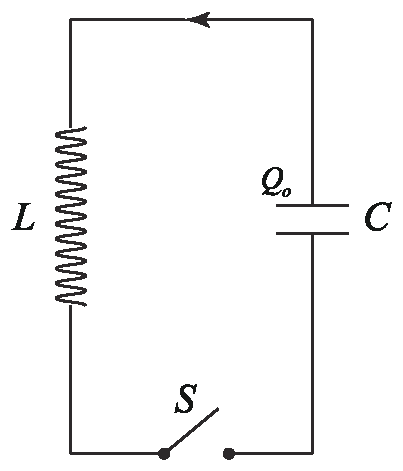
\includegraphics[width = 0.3\textwidth]{images/alt-current-3.pdf} 
\end{flushright}

\tagged{student}{\vspace*{3cm}}
\begin{taggedblock}{teacher}
\noindent
解析:LC回路,当做例题让同学自己发现其中的规律。
\end{taggedblock}
\end{example}
%%%%%%%%%%%%%%%%%%%%%%


%%%%%%%%%%%%%%%%%
\begin{example}

用回旋加速器加速质量为$m$,带电量为$q$的粒子,加速器的磁感应强度为$B$,用$LC$振荡器作为高频电源对粒子加速,该振荡器的电感$L$和电容$C$的乘积是多少?
\tagged{student}{\vspace*{2cm}}
\begin{taggedblock}{teacher}
\noindent
解析:振荡的频率要与带电粒子是磁场中运动的频率一致
\[
\frac{2 \pi m}{B q} = 2\pi \sqrt{LC},\qquad LC = \frac{m^2}{B^2q^2}.
\]
\end{taggedblock}
\end{example}
%%%%%%%%%%%%%%%%%%%%%%

\section{交流电路的矢量图解}

\section{变压器}
通过相同电阻$R$的导线,我们知道导线上消耗的电功率正比于导线上分得的有效电压的平方,反比于导线的电阻:
\begin{equation}
P_R = \frac{(\Delta U)_{eff}^2}{R},
\end{equation}
而也可以表示成传输的总有效电流的平方与导线电阻的乘积:
\begin{equation}
P_R = I_{eff}^2 R
\end{equation}
简单的分析可知从发电场到各个用户的输电过程中,有效电流越小,则消耗在传输线路中的电功率就越小,这就是实践上普遍采用高压输电的原理:由于传输总功率$P=U_{eff} I_{eff}$在传输的过程中不变,提高传输电压意味着减小了总传输电流,从而降低了在传输线路上的损耗。
当高压电进入城市以后,也需要通过一定的技术手段降低交流电的电压,而完成这些功能的电学装置就被称为{\heiti 变压器}(transformer)。

利用互感现象制成的变压器就是互感变压器,其基本原理如图所示。
左边线圈接入待变压的电源,叫做{\heiti 主线圈}(primary winding),右边接入负载,叫{\heiti 副线圈}(secondary winding),变压器中间的铁芯选用磁导率较大的材料,能够使磁场尽量只局域在铁芯中。
对于理想变压器,磁场全部局域在铁芯中。于是当原线圈中电流发生变化时,主、副线圈中的总磁通都会发生变化,从而在原、副线圈中产生感应电动势。

根据法拉第电磁感应定律,可以得到原、副线圈中感应电动势
\[
\mathcal{E}_1 = n_1\frac{\Delta \Phi_1}{\Delta t},\qquad \mathcal{E}_2 = n_1\frac{\Delta \Phi_2}{\Delta t}
\]
其中$n_{1,2}$分别是原、副线圈的匝数,$\Phi_{1,2}$则是两线圈中通过一个线圈的磁通量。
最理想的情况下,假设主线圈中产生的磁感线全部由铁芯传递到副线圈,并且主、副线圈的电阻小到可以忽略,这样$\Delta\Phi_1 = \Delta \Phi_2$,两线圈中的电动势之间满足:
\begin{equation}
\frac{U_1}{U_2} = \frac{n_1}{n_2},
\end{equation}
这就是{\heiti 电压变比条件}(voltage ratio condition)如果我们进一步假设变压器自身的能量损失可以忽略不计,则有
\begin{equation}
P_1 =P_2, \qquad I_1U_1 = I_2U_2,\qquad \frac{I_1}{I_2} = \frac{n_2}{n_1}
\end{equation}
这就是{\heiti 电流变比条件}(current ratio condition)。
满足以上两个关系的变压器也被称作{\heiti 理想变压器}(ideal transformer)。



%%%%%%%%%%%%%%%%%
\begin{example}

通过计算回答以下几个问题:

1. 某一台发电机的输出功率为$7.8\pow{5}\unit{W}$,要将其送至某小镇,输电线的电阻为$12\Omega$。
用$5\unit{kV}$和$20\unit{kV}$两种电压输送,求每种情况下输电线的发热功率占总功率的百分比。

2. 若发电机输出电压为$1000\unit{V}$,采用$20\unit{kV}$的电压输送,则所用变压器原、副线圈匝数比应为1:\kong\kong ?

3. 由于传输线电阻的存在,到达小镇后,高压线的电压已经减少为多少了?

4. 要将到达小镇的高压电变为$220\unit{V}$市电,问变压器原、副线圈匝数比约为\kong :1
\tagged{student}{\vspace*{4cm}}
\begin{taggedblock}{teacher}
\newline
解析:1.设消耗的功率为P’:\[I_1=156A,P'=156^2*12\]
\[\eta=37.44\%\]
\[I_2=39A,P'=39^2*12\]
\[\eta=2.34\%\]
2.200
\\3.19532V
\\4.88
\end{taggedblock}
\end{example}
%%%%%%%%%%%%%%%%%%%%%%


%%%%%%%%%%%%%%%%%
\begin{example}

一变压器如下图,除线圈分别有内阻$r_1$、$r_2$外,可以看做理想变压器(磁场全部局域在铁芯中,且传递过程中不损失能量),主线圈接入交流电的有效值为$U$,线圈匝数分别为$n_1$和$n_2$。
试求当负载为纯电阻$R $时,主副线圈中的电流有效值。
\begin{flushright}
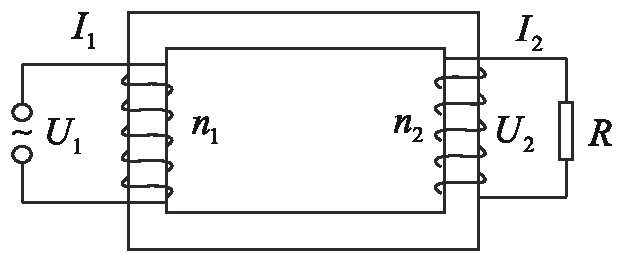
\includegraphics[width = 0.4\textwidth]{images/mag-42.pdf} 
\end{flushright}
\tagged{student}{\vspace*{4cm}}
\begin{taggedblock}{teacher}
\noindent
解析:
\[I_1=\frac{U_1}{r_1+\frac{n_1^2}{n_2^2}(R+r_2)}\]

\[I_2=\frac{n_1}{n_2}I_1\]
\end{taggedblock}
\end{example}
%%%%%%%%%%%%%%%%%%%%%%

\section{*整流、滤波和稳压}

虽然交流电有其独特的优势,但很多电子设备依然使用直流电作为其工作电流,这时就需要通过一定的手段将交流电转变为直流电,这一操作称之为{\heiti 整流}(rectification)。
利用二极管的单向导电性可以帮助完成整流,理想的二极管正向电阻为零,可看成理想导线,反向电阻无限大,可看成断路。
通过以下几个例子可以看出整流的过程:


%%%%%%%%%%%%%%%%%
\begin{example}

【半波整流】如图所示的半波整流电路,其中$B$是变压器,$D$是理想二极管,$R$是一个普通电阻。
如果输入电压随时间的变化关系为已知时,在下面坐标中定性地画出回路中电流随时间的变化关系。
\begin{center}
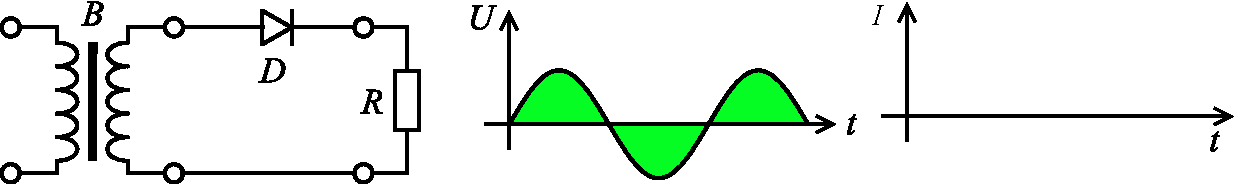
\includegraphics[width = 0.9\textwidth]{images/alt-current-7.pdf} 
\end{center}
\tagged{student}{\vspace*{4cm}}
\begin{taggedblock}{teacher}
\noindent
解析:略
\end{taggedblock}
\end{example}
%%%%%%%%%%%%%%%%%%%%%%



%%%%%%%%%%%%%%%%%
\begin{example}

【桥式整流电路】如图所示的是桥式整流电路,其中四个二极管均可看成理想二极管,当输入电压为正弦交流电时,在右图中画出输出电压随时间的变化关系。
\begin{center}
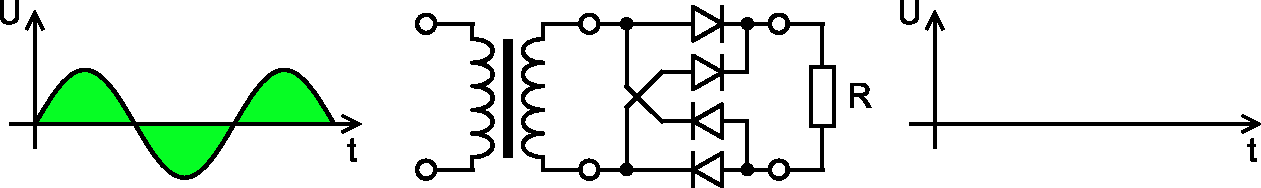
\includegraphics[width = 0.9\textwidth]{images/alt-current-8.pdf} 
\end{center}
\tagged{student}{\vspace*{4cm}}
\begin{taggedblock}{teacher}
\noindent
解析:略
\end{taggedblock}
\end{example}
%%%%%%%%%%%%%%%%%%%%%%


从上面几个例子可以看出,经过简单整流以后的交流电与通常的直流电还是有较大的差别,虽然电压不再有反向分量,但随时间的变化关系依然剧烈,不适合实际的使用需求。
将脉动的直流电转化为输出电压较为平稳直流电的过程称为{\heiti 滤波}(filtration)。
滤波的核心思想是尽可能地去掉电压的交流成份,但保留其中的直流成分,经过滤波之后的输出电压将看上去更加平稳。
通过以下几个例子来掌握简单的滤波原理和电路。


%%%%%%%%%%%%%%%%%
\begin{example}

【电容滤波】下图是半波整流之后接一个电容滤波电路,试定性地给出滤波后的通过$R$的电流随时间的变化关系,分析滤波效果和电容大小的关系。
\begin{center}
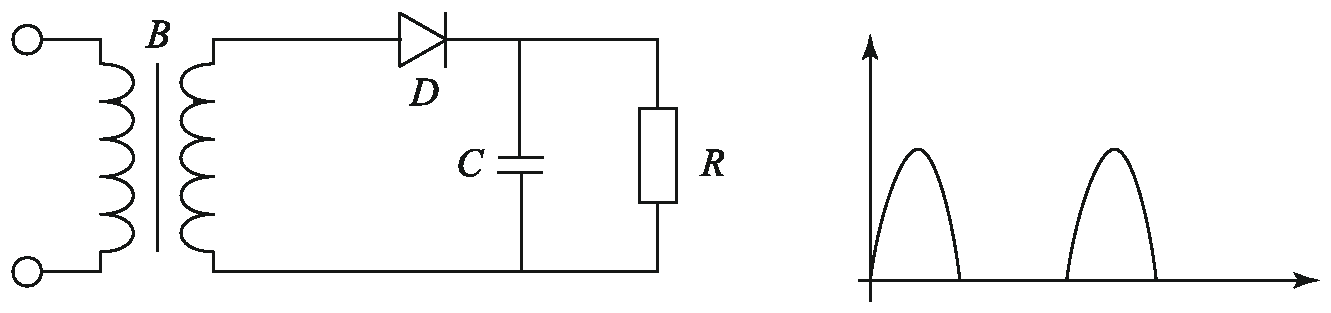
\includegraphics[width = 0.9\textwidth]{images/alt-current-9.pdf} 
\end{center}

\tagged{student}{\vspace*{4cm}}
\begin{taggedblock}{teacher}
\noindent
解析:利用电容可通过交流、阻隔直流的性质做定性画图。
电容越大,容抗越小,交流电更喜欢从电容通过,所以滤波效果更佳。
\end{taggedblock}
\end{example}
%%%%%%%%%%%%%%%%%%%%%%


%%%%%%%%%%%%%%%%%
\begin{example}
可否利用电感对交流电产生感抗,对直流电可看成导线这样的性质设计一个简单滤波电路,并定性地给出滤波效果和电感大小的关系。

\tagged{student}{\vspace*{4cm}}
\begin{taggedblock}{teacher}
\noindent
解析:全波整流电路中和。‘电阻串联一个电感可完成滤波,而且电感越大,滤波效果越好。
\end{taggedblock}
\end{example}
%%%%%%%%%%%%%%%%%%%%%%

仅靠整流和滤波可以得到几乎平稳的输出电压,但是精密的电子元件通常需要更加平稳的电源供应,这时就需要引入对电压更加精密的控制手段,技术上称之为{\heiti 稳压}(voltage stabilitation)。
电路的稳压通常需要借助半导体的特性以及电路的反馈机制来完成,感兴趣的同学可以通过阅读相关资料了解稳压的原理及典型电路。


